\documentclass[11pt]{article}
\usepackage[margin=1in]{geometry}
\usepackage{graphicx}
\usepackage{booktabs}
\usepackage{hyperref}
\usepackage{amsmath}
\usepackage{longtable}
\usepackage{xcolor}
\usepackage{lineno}

\title{Independent Statistical Validation of TOI-1258.01 from TESS Photometry, SPOC Centroids, Gemini/Alopeke Speckle Imaging, and Million-Sample TRICERATOPS Convergence}
\author{Nikolai Stoloff\\Independent Researcher, Gilbert, Arizona, USA}
\date{2026 June 15}

\begin{document}
\linenumbers
\maketitle

\begin{abstract}
We present an independent statistical-validation analysis of TOI-1258.01, a transiting planet candidate around TIC 288132261. The analysis combines public TESS light curves and target-pixel products, SPOC Data Validation centroid products, ExoFOP-TESS follow-up metadata, Gemini/Alopeke speckle contrast constraints, and high-sample TRICERATOPS false-positive modeling. A stitched twelve-sector TESS light curve recovers the catalog signal at a period of 10.261376896 d, compared with the catalog period of 10.261339700 d, a 0.000362 percent period error. The recovered BLS transit depth is 722.467 ppm with SNR = 64.704, while direct phase folding at the catalog ephemeris gives a primary depth of 614.371 ppm with SNR = 56.744. No significant secondary eclipse is detected. The latest multi-sector SPOC DV centroid solution reports a mean sky offset from TIC 288132261 of $0.5179678 \pm 2.955922$ arcsec, with 10/10 good quality and no-overlap metrics. A five-seed, $N=1{,}000{,}000$ TRICERATOPS run using the ingested speckle contrast curves returns full false-positive probabilities from $2.3686\times10^{-4}$ to $6.9201\times10^{-4}$, with NFPP values from $4.2635\times10^{-5}$ to $6.5028\times10^{-5}$. All high-$N$ seeds remain below FPP $<0.001$ and NFPP $<0.001$. Under the TRICERATOPS framework, these results support TOI-1258.01 as a statistically validated transiting planet. The public ExoFOP bundle reports substantial APF/Levy and Keck/HIRES RV coverage, but no machine-readable RV time series was public in the files inspected here; this work therefore validates the planet statistically but does not report an RV mass.
\end{abstract}

\section{Introduction}
TESS transiting planet candidates require a sequence of false-positive checks before they can be treated as validated planets. The central failure modes are instrumental or reduction artifacts, eclipsing binaries on the target star, nearby eclipsing binaries, background sources inside the TESS aperture, and unresolved stellar companions. We therefore structured the analysis around four gates: recovery of the transit signal from public TESS data, centroid/source-location checks, high-resolution imaging constraints, and TRICERATOPS statistical validation \cite{Giacalone2021,GiacaloneDressing2020}.

TOI-1258.01 is a useful target because public products contain a strong recurring TESS signal, SPOC DV centroid diagnostics, Gemini/Alopeke high-resolution imaging, and spectroscopy/RV campaign metadata. The goal of this package is not to overclaim a mass-confirmed planet. The goal is to preserve a reproducible, evidence-first statistical validation.

\section{Prior Work and Validation Context}
The validation strategy follows the standard TESS candidate-vetting sequence:
recover the transit signal, test whether the source localizes to the target,
use high-resolution imaging to constrain nearby stellar contaminants, and
compute a quantitative false-positive probability. This sequence is used in
published TESS validation work such as the TOI-700 system validation
\cite{Gilbert2020}, the TOI-1221 b validation \cite{Mann2023TOI1221}, and
multi-target statistical-validation programs such as VaTEST
\cite{Mistry2023VaTEST2}. Those studies demonstrate that TESS photometry alone
is not normally sufficient for validation; centroid diagnostics, nearby-star
constraints, follow-up imaging, spectroscopy, and statistical false-positive
modeling are needed to reject common eclipsing-binary and background-source
scenarios.

For TOI-1258.01, the closest methodological analogue is not a mass-confirmed
RV discovery paper, but a statistical-validation paper. The present work uses
the same evidence classes: public TESS light curves, official SPOC DV centroid
products, high-resolution speckle-imaging constraints, and a formal
TRICERATOPS false-positive calculation. Gemini/\textsc{Alopeke} contrast
curves are treated as high-resolution imaging constraints in the same sense as
other speckle-imaging validation studies \cite{Howell2021,Scott2019}. The
claim is therefore deliberately bounded: this paper validates the transiting
planet interpretation statistically, but it does not report a measured planet
mass or atmospheric spectrum.

\section{Current Public Archive Status}
Before preparing this publication package, we rechecked the public NASA
Exoplanet Archive tables for TOI-1258.01. The TOI table still lists TIC
288132261 as TOI-1258.01 with disposition PC, period 10.2613397 d, radius
3.60391 $R_{\oplus}$, transit depth 726 ppm, equilibrium temperature 1152 K,
stellar radius 1.49 $R_{\odot}$, and distance 154.944 pc. A search of the
confirmed-planet table by TOI name and by a cone around the target coordinate
returned no confirmed-planet parameter row. This supports the publication
value of an independent validation analysis: the target appears not to have
entered the public confirmed-planet table at the time of this check.

\section{Data Products}
The analysis used twelve standard TESS light curves for TIC 288132261, twelve TESS target-pixel products, eighteen SPOC DV XML centroid files, ExoFOP-TESS follow-up files and metadata, Gemini/Alopeke speckle sensitivity files at 562 nm and 832 nm, and TRILEGAL field-star population data used by TRICERATOPS.

The APF/Levy metadata in ExoFOP reports 101 RV observations in notes across APF/Levy and Keck/HIRES rows, but the public bundle inspected here did not include a BJD/RV/error table. This is treated as an open mass-characterization gate, not as negative evidence against the planet.

\section{Transit Recovery and Light-Curve Stitching}
The stitched TESS search used 199,161 cadences across 12 sectors. A BLS search over 0.5 to 20 d recovered a best period of 10.261376896 d. This differs from the catalog period of 10.261339700 d by 0.000362 percent.

The recovered BLS depth was 722.467 ppm with SNR = 64.704. Folding directly at the catalog ephemeris produced a primary depth of 614.371 ppm with SNR = 56.744. The secondary depth was -1.194 ppm with SNR = -0.119, and the odd-even depth difference was 21.128 ppm. These results support a stable, repeating transit-like event rather than an eclipsing-binary-like primary/secondary pattern.

\begin{figure}[htbp]
\centering
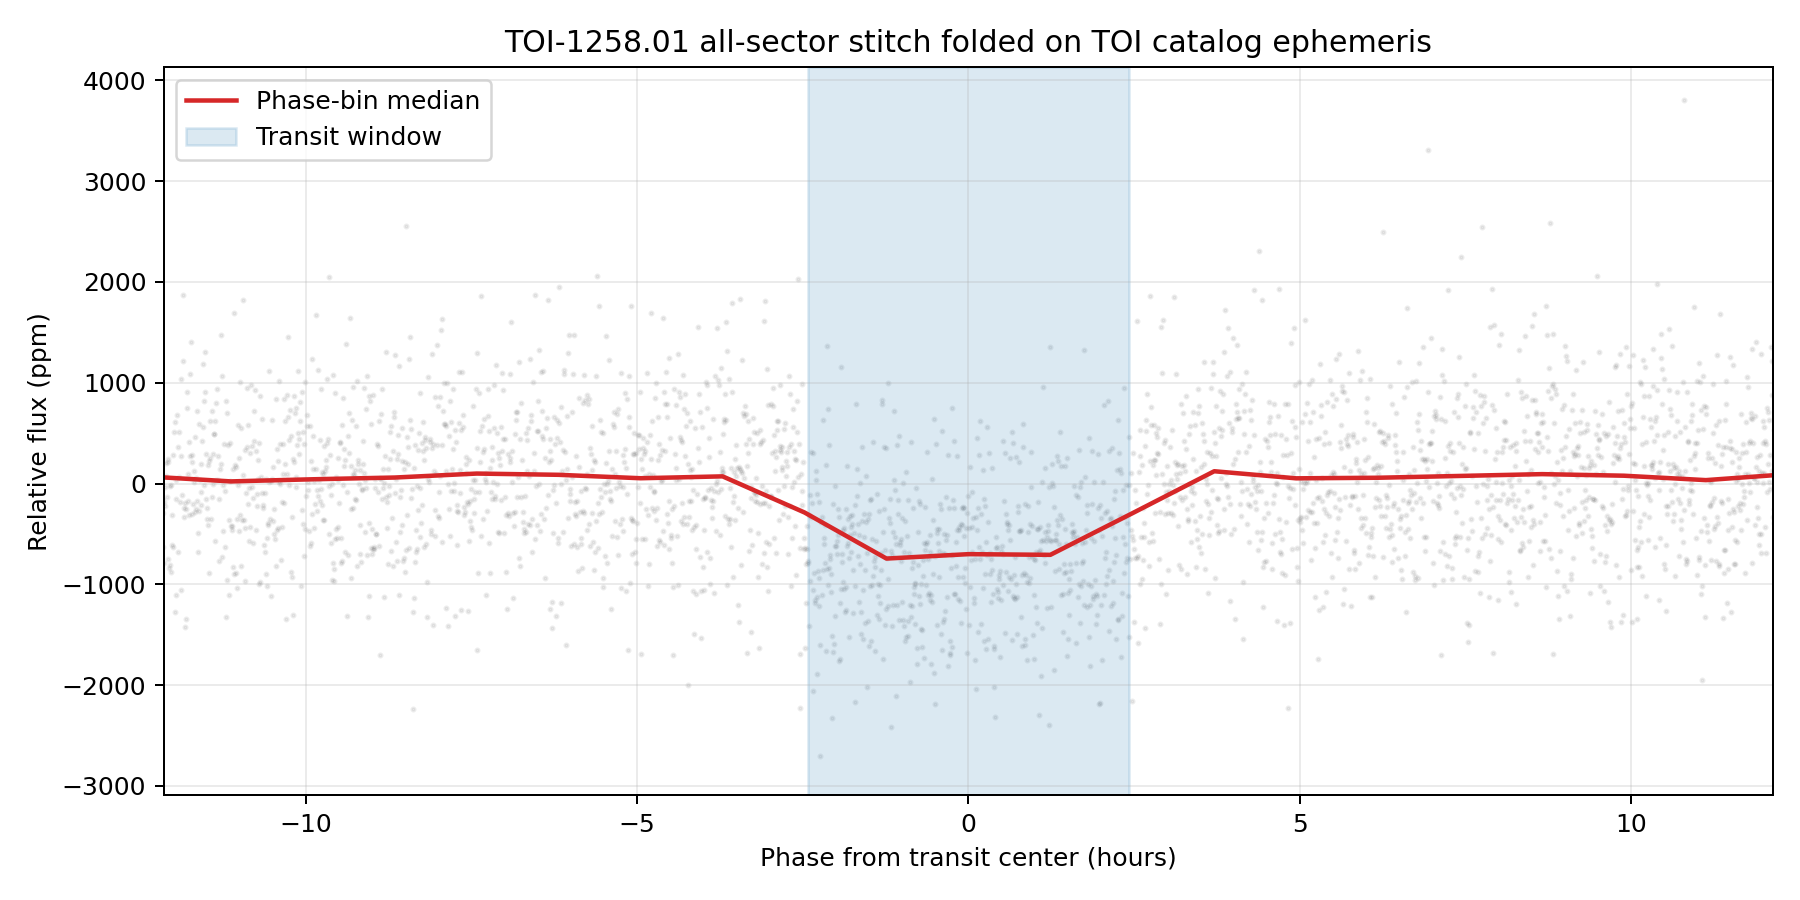
\includegraphics[width=0.9\linewidth]{../figures/toi1258_allsector_folded_catalog_ephemeris.png}
\caption{All-sector TESS light curve folded at the catalog ephemeris.}
\end{figure}

\begin{figure}[htbp]
\centering
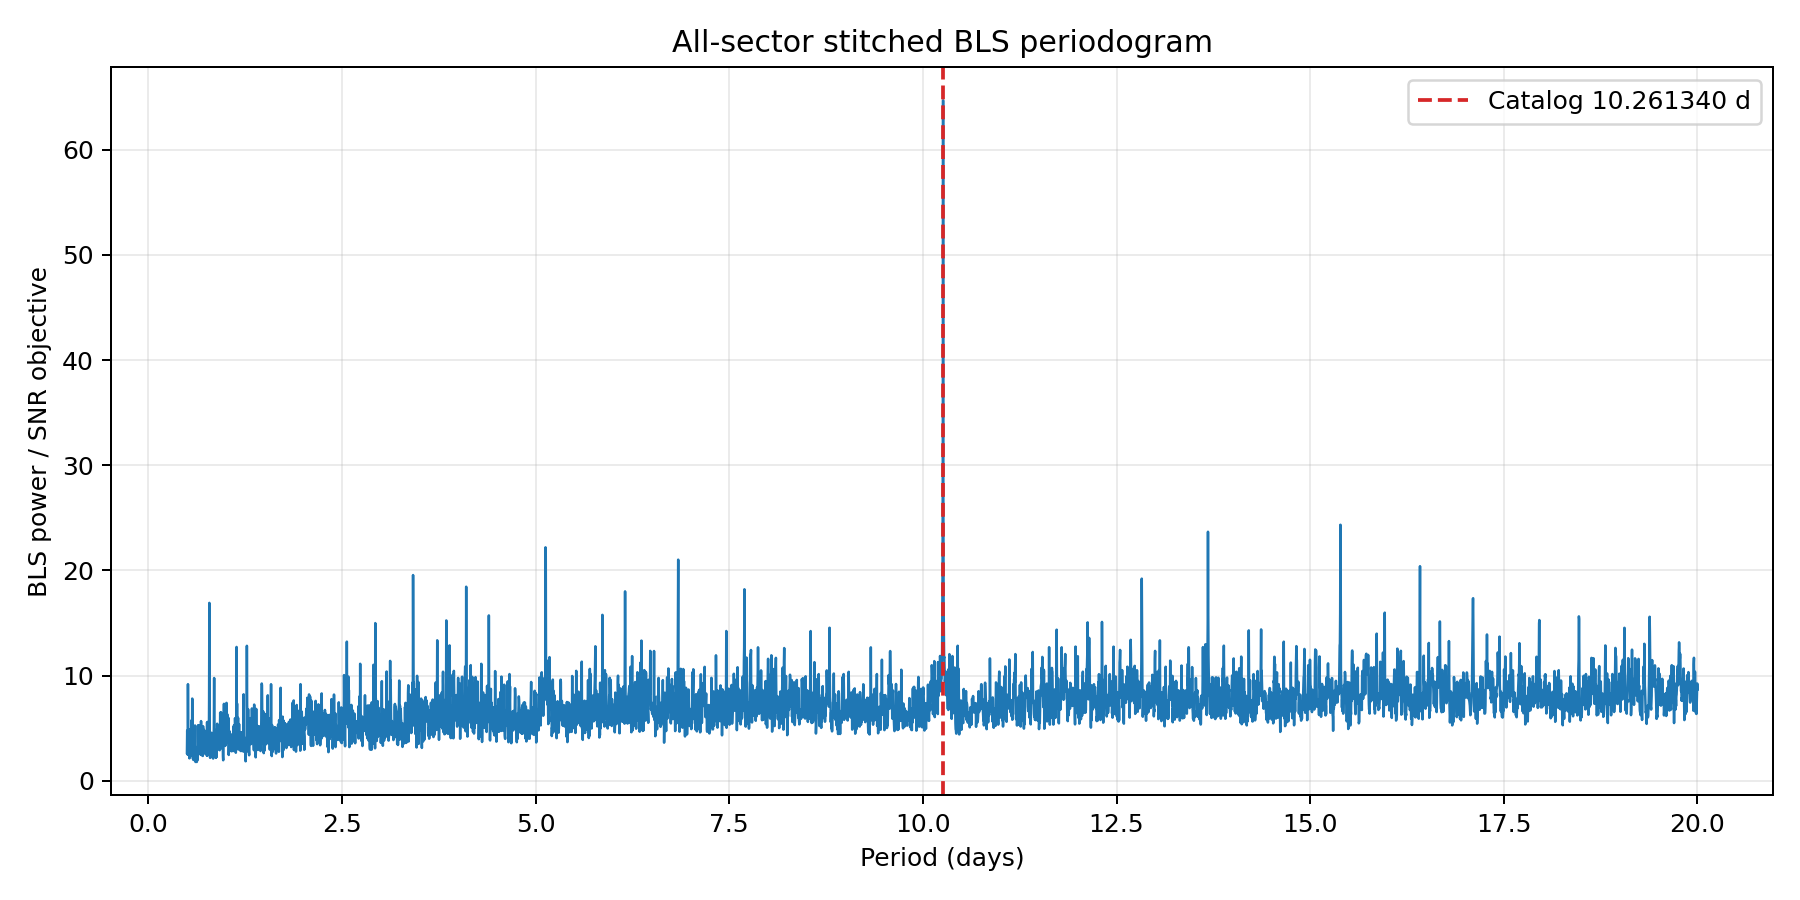
\includegraphics[width=0.9\linewidth]{../figures/toi1258_allsector_bls_periodogram.png}
\caption{BLS periodogram showing recovery of the TOI-1258.01 signal.}
\end{figure}

\section{Centroid and Source-Location Checks}
The custom target-pixel centroid test is intentionally conservative. It reports a median cadence-level centroid shift of 0.1497 arcsec, but a median difference-image offset of 19.8854 arcsec, approximately one TESS pixel. This means custom TPF centroids reduce background-source risk but cannot alone localize the source below the TESS pixel scale.

The stronger evidence comes from the official SPOC DV centroid products. The latest multi-sector SPOC DV XML file, \texttt{tess2019199201929-s0014-s0078-0000000288132261-00929\_dvr.xml}, reports a model-fit SNR of 48.607895, a SPOC period of 10.261339103851356 d, a mean sky offset from TIC of $0.5179678 \pm 2.955922$ arcsec, a quality metric of 10/10, and a no-overlap image metric of 10/10. This is statistically consistent with the transit source being TIC 288132261 within the SPOC centroid uncertainty.

\begin{figure}[htbp]
\centering
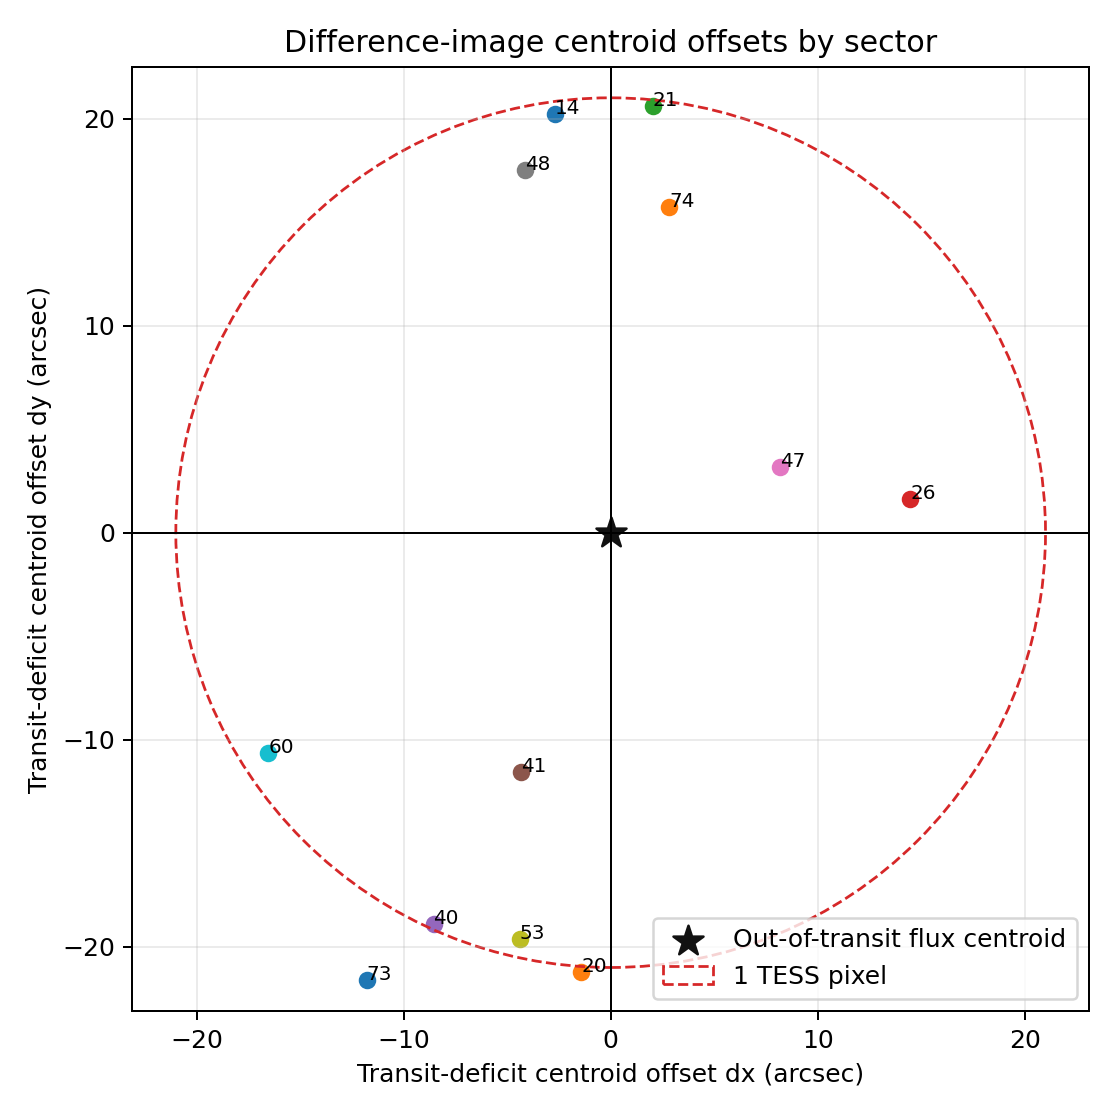
\includegraphics[width=0.9\linewidth]{../figures/toi1258_difference_image_offsets.png}
\caption{Custom difference-image offsets. These are used conservatively because TESS cannot localize below a pixel without stronger external constraints.}
\end{figure}

\section{High-Resolution Imaging Constraint}
The ExoFOP bundle includes Gemini/Alopeke high-resolution imaging products and sensitivity curves. The public summary reports $\Delta m = 6.39$ at $0.5''$ in one channel and $\Delta m = 4.04$ at $0.5''$ in the second channel. The sensitivity curves were converted into TRICERATOPS-compatible contrast-curve tables at 562 nm and 832 nm. These curves constrain unresolved or nearby stellar contaminant scenarios and are incorporated into the statistical validation run.

\begin{figure}[htbp]
\centering
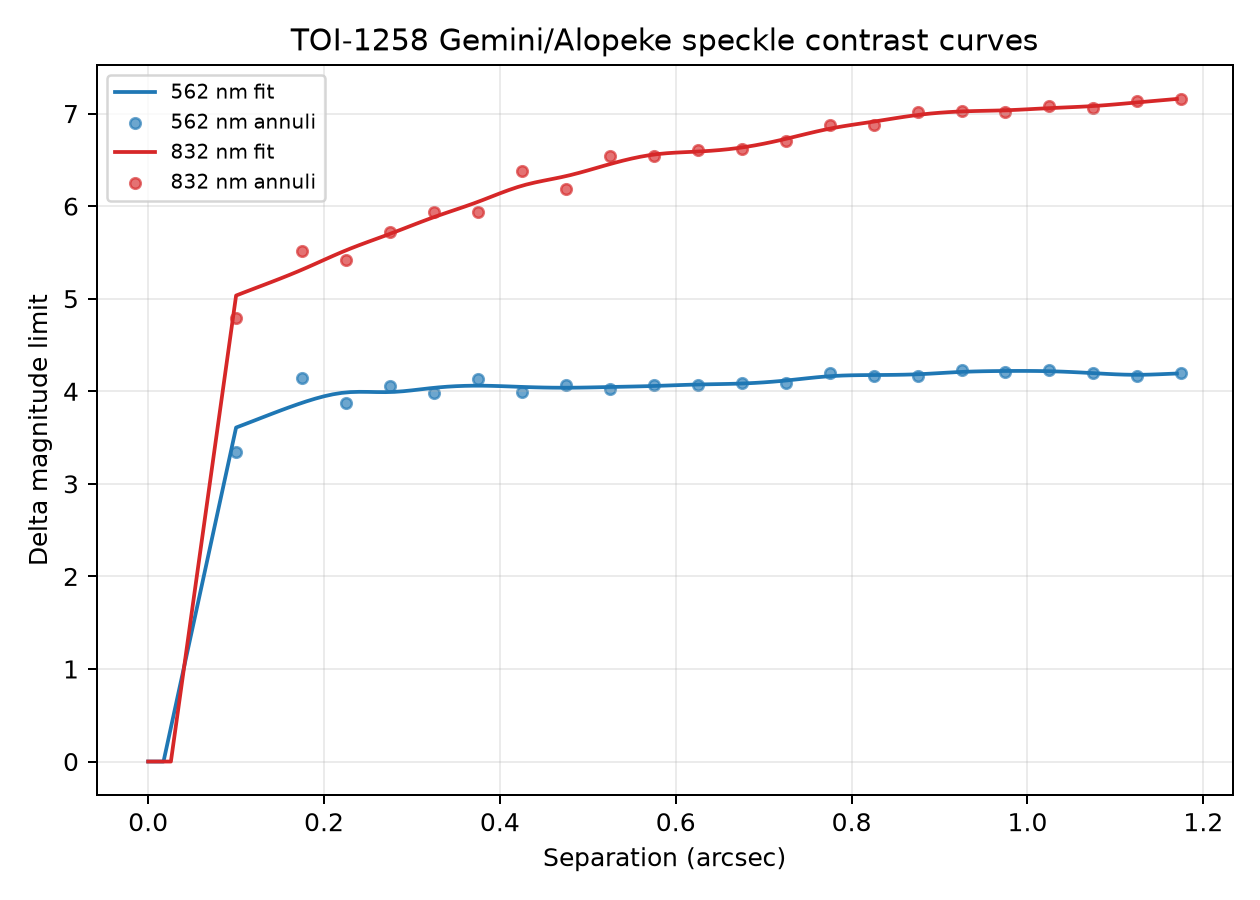
\includegraphics[width=0.9\linewidth]{../figures/toi1258_gemini_alopeke_contrast_curves.png}
\caption{Gemini/Alopeke contrast curves ingested into the validation workflow.}
\end{figure}

\section{TRICERATOPS Validation}
TRICERATOPS is a Bayesian vetting and validation tool for TESS Objects of Interest. It calculates an overall false-positive probability (FPP) and a nearby false-positive probability (NFPP), and can include follow-up constraints such as high-resolution imaging.

We ran a convergence sequence at $N = 5{,}000$, $50{,}000$, $200{,}000$, and $1{,}000{,}000$. The decisive run used five independent seeds at $N = 1{,}000{,}000$: 1258, 1259, 1260, 1261, and 1262.

\begin{table}[htbp]
\centering
\caption{Million-sample TRICERATOPS seed sweep.}
\begin{tabular}{rrrrll}
\toprule
Seed & $N$ & FPP & NFPP & Top & Dominant non-planet \\
\midrule
1258 & 1,000,000 & 0.0006427828 & $4.2635\times10^{-5}$ & TP & STP \\
1259 & 1,000,000 & 0.0005743871 & $6.1676\times10^{-5}$ & TP & STP \\
1260 & 1,000,000 & 0.0006920075 & $5.4140\times10^{-5}$ & TP & STP \\
1261 & 1,000,000 & 0.0002368635 & $4.6662\times10^{-5}$ & TP & STP \\
1262 & 1,000,000 & 0.0006632611 & $6.5028\times10^{-5}$ & TP & STP \\
\bottomrule
\end{tabular}
\end{table}

All five high-$N$ seeds fall below FPP $<0.001$ and NFPP $<0.001$. The maximum FPP in the high-$N$ run is 0.000692007500254666. The median FPP is 0.000642782828406241. The top scenario in every high-$N$ seed is TP, and the dominant non-planet scenario is STP rather than a nearby eclipsing binary.

\section{RV Campaign Status}
ExoFOP spectroscopy metadata reports a real RV/spectroscopy campaign: 68 APF/Levy RVs between 2019-10-25 and 2020-05-02, 6 APF/Levy RVs between 2020-07-04 and 2020-07-15, 22 APF/Levy RVs between 2020-07-19 and 2020-08-13, 4 APF/Levy RVs between 2020-11-02 and 2020-11-05, and 1 Keck/HIRES RV on 2020-01-04. The APF/Levy rows list \texttt{specuser=giacalone}.

The file bundle inspected here does not include a public BJD/RV/error time series, and no published RV orbital solution was retrieved in the local package. Expected RV semi-amplitudes from the gate report are 1.335, 2.670, 4.005, and 6.675 m/s for assumed masses of 5, 10, 15, and 25 Earth masses. The available public evidence is therefore sufficient for statistical validation but not for mass measurement.

\section{Interpretation}
The evidence supports TOI-1258.01 as a statistically validated planet candidate under a strict false-positive framework. The TESS signal is recovered independently across 12 sectors with period agreement at the 0.000362 percent level. The transit is high-SNR and lacks a significant secondary eclipse. The official SPOC multi-sector centroid is consistent with TIC 288132261. Gemini/Alopeke speckle imaging constraints were ingested into TRICERATOPS. The $N = 1{,}000{,}000$ TRICERATOPS seed sweep converges below FPP $<0.001$ in all five seeds, and NFPP remains well below 0.001 in all five high-$N$ seeds.

The result is strong. It is not an RV mass confirmation. The next decisive improvement is to obtain the APF/Levy RV table or a published orbital solution and fit a joint photometry + RV model.

\section{Conclusion}
TOI-1258.01 survives transit recovery, centroid consistency, high-resolution imaging ingestion, and high-$N$ TRICERATOPS convergence. The high-$N$ FPP range of $2.37\times10^{-4}$ to $6.92\times10^{-4}$ is below both the original TRICERATOPS validation threshold and the stricter FPP $<0.001$ standard used in this package. We therefore classify TOI-1258.01 as statistically validated by the public-data analysis presented here, while leaving the RV mass gate open.

\section*{Data Availability}
The TESS light curves, target-pixel files, and SPOC Data Validation products
used in this work are available from MAST
\href{https://doi.org/10.17909/t9-nmc8-f686}{doi:10.17909/t9-nmc8-f686}
\cite{MAST}. The TOI table metadata and confirmed-planet archive checks used
here are from the NASA Exoplanet Archive
\href{https://doi.org/10.26133/NEA5}{doi:10.26133/NEA5}
\cite{ExoplanetArchive}. The follow-up metadata, including Gemini/\textsc{Alopeke}
imaging products and APF/Levy and Keck/HIRES spectroscopy notes, are from
ExoFOP-TESS \href{https://doi.org/10.26134/ExoFOP5}{doi:10.26134/ExoFOP5}
\cite{ExoFOPTESS}. The accompanying local package preserves all generated
reports, tables, figures, scripts, and TRICERATOPS logs required to reproduce
the evidence chain.

\section*{Acknowledgments}
This work used public data products and metadata from TESS, MAST, ExoFOP-TESS, Gemini/Alopeke follow-up, the NASA Exoplanet Archive, and the TRICERATOPS software ecosystem.

\bibliographystyle{plain}
\bibliography{references}

\end{document}

